% Generated by pipeline/paper/scripts/make_result_figures.py. Do not edit by hand.
% Indicative per-record CLI. One run per proteome. Both outcomes are EXACT.
% Shared figure style. Input once; a second input is a no-op.
\ifdefined\actsplotsready
\else
  \def\actsplotsready{1}
  \colorlet{actsteal}{teal!72!black}
  \colorlet{actstealfaint}{teal!16}
  \colorlet{actsorange}{orange!88!black}
  \colorlet{actsink}{black!80}
  \colorlet{actsghost}{black!45}
  \colorlet{actsfail}{red!62!black}
  \colorlet{actsrule}{black!50}
  \usetikzlibrary{intersections}
  \usepgfplotslibrary{fillbetween,groupplots}
  \pgfplotsset{
    acts/.style={
      font=\scriptsize\sffamily,
      tick label style={font=\scriptsize\sffamily},
      label style={font=\scriptsize\sffamily},
      legend style={
        font=\scriptsize\sffamily,
        draw=none,
        fill=none,
        cells={anchor=west},
        inner sep=1pt,
        column sep=6pt
      },
      legend cell align=left,
      scale only axis,
      clip=false,
      axis line style={actsrule},
      tick style={actsrule},
      tick align=outside,
      axis lines=left,
      xmajorgrids=true,
      major grid style={black!7},
      ymajorgrids=false,
      every node/.append style={font=\scriptsize\sffamily, inner sep=1.5pt},
      every axis plot/.append style={line join=round, line cap=round},
    },
  }
  \tikzset{
    actlab/.style={
      font=\scriptsize\sffamily,
      fill=white,
      fill opacity=0.92,
      text opacity=1,
      inner sep=1.35pt,
      outer sep=0.5pt,
    },
  }
\fi

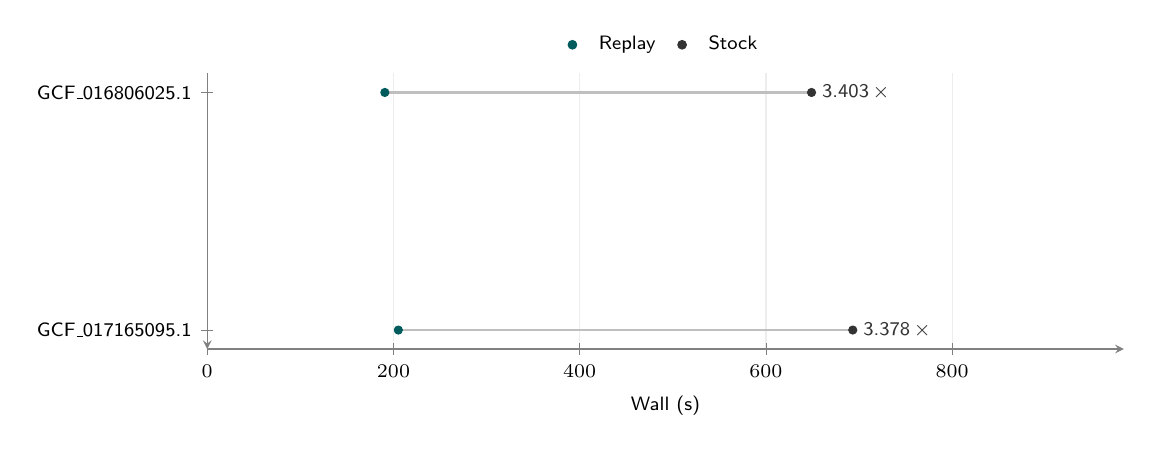
\begin{tikzpicture}
\begin{axis}[
  acts,
  width=0.96\columnwidth,
  height=3.50cm,
  xmin=0, xmax=984.365,
  xtick={0,200,400,600,800},
  xlabel={Wall (s)},
  symbolic y coords={r0,r1},
  ytick={r0,r1},
  y dir=reverse,
  yticklabels={{GCF\_016806025.1},{GCF\_017165095.1}},
  enlarge y limits=0.08,
  legend style={at={(0.5,1.04)}, anchor=south, legend columns=2},
]
\addplot[draw=none, forget plot] coordinates {(0,r0) (0,r1)};
\addlegendimage{only marks, mark=*, mark size=1.55pt, draw=actsteal, fill=actsteal}
\addlegendentry{Replay}
\addlegendimage{only marks, mark=*, mark size=1.55pt, draw=actsink, fill=actsink}
\addlegendentry{Stock}
% connector black!25
\draw[black!25, line width=0.9pt] (axis cs:190.6952,r0) -- (axis cs:648.94162,r0);
\draw[black!25, line width=0.9pt] (axis cs:205.20091,r1) -- (axis cs:693.21456,r1);
% source: exact_replay/costpass_measured.json e2.wall_s and stock.wall_s
\addplot[only marks, mark=*, mark size=1.45pt, draw=actsteal, fill=actsteal, forget plot] coordinates {(190.6952,r0) (205.20091,r1)};
% source: exact_replay/costpass_measured.json e2.wall_s and stock.wall_s
\addplot[only marks, mark=*, mark size=1.45pt, draw=actsink, fill=actsink, forget plot] coordinates {(648.94162,r0) (693.21456,r1)};
\node[actlab, anchor=west, text=actsink, xshift=2pt] at (axis cs:648.94162,r0) {3.403\,$\times$};
\node[actlab, anchor=west, text=actsink, xshift=2pt] at (axis cs:693.21456,r1) {3.378\,$\times$};
\end{axis}
\end{tikzpicture}
